\section{\label{sec:Style}Style \& Grammar}

\begin{itemize}[label=$\Box$]
\item Use the active voice. If you use the passive voice, it is very hard to tell the difference between what you personally worked hard to do in your experiment, vs.\ what you are citing as a prior result.
\item Avoid pronouns if at all possible (e.g.\ not ``that'' but ``that voltage signal'').
% \item The word ``this'' must always be followed by a noun, so that its reference is explicit. Not: This is a fast reaction; This leads us to conclude But: This reaction is fast; This observation leads us to conclude
\item Use adjectives if there is any doubt (e.g.\ not ``the modulation'' but ``the $z$ modulation'').
% \item Describe experimental results uniformly in the past tense (e.g.\ not ``Landau levels appear when $B$ is applied'' but ``Landau levels appeared when $B$ was applied'').
% \item Complete all comparisons (e.g.\ not ``The signal was stronger at 2 Kelvin'' but ``The signal was stronger at 2 Kelvin than at 4 Kelvin'').
\item Define all acronyms and symbols at first use; then use the acronym consistently from that point on.
\item Do not use the word ``significantly'' -– unless you mean it in the true statistical sense and are prepared to back it up quantitatively.
%\item Journals also typically don't like the words ``new'' or ``novel''. It can be ok to use these words sparingly in a first submission, to catch the editor's or referee's attention, but these words should not be overused.
\item Remove redundancy, including redundancy between main text and figure captions. When in doubt, the information probably belongs in the caption but not the main text.
\item Check that all equations are dimensionally correct.
\item For each equation, define all symbols in a previous equation or in the surrounding text.
\item Report each quantity consistently throughout the text (e.g.\ don't exaggerate a quantity in one place, give an exact version of the same quantity in another place, and round to the nearest 100 in a third place).
\item Check that all numbers have units.
\item Use reasonable significant figures, report errors where appropriate, and clearly explain the method of error determination.
\item When in doubt, check examples (e.g.\ if you wonder whether acronyms are appropriate in the abstract, check a few recent published examples in your target journal).
\item ``Only'' can be an adjective or an adverb, so its meaning can be ambiguous. It should be placed immediately before the noun, adjective, or verb that it is modifying. For example ``I only bought groceries at the store'' means I didn't run, jump, dance, or sing at the store, I only bought. But ``I bought only groceries at the store'' means I didn't buy valves or screws at the store.
\item ``Its'' is possessive;\\ ``it's'' is a contraction of ``it'' and ``is''.
\item ``which'' vs.\ ``that'': \url{http://www.writersdigest.com/online-editor/which-vs-that}
\item ``fewer'' vs.\ ``less'': \url{http://www.quickanddirtytips.com/education/grammar/less-versus-fewer}
\item ``affect'' vs.\ ``effect'': \url{http://grammarist.com/usage/affect-effect/}
\item See additional tips from Prof.\ Margo Seltzer: \url{http://www.seltzer.com/margo/pet-peeves/}
\end{itemize}

\section{\label{sec:Figures}Figures}

\ptitle{Figure style} It is worth taking 2-3 hours to read the definitive guide to ``The Visual Display of Quantitative Information'' by Edward Tufte \cite{TufteVisualDisplay2001}. Tufte defines several metrics for figure optimization:

\vspace{2mm}
\noindent $\displaystyle{\text{Data-ink ratio} = \frac{\text{data-ink}}{\text{total ink used to print the graphic}}}$
\vspace{-1mm}
\begin{eqnarray}
\nonumber & = 1.0 - & \text{fraction of a graphic that can be} \\[-2pt]
\nonumber & & \text{erased without loss of data-information}
\end{eqnarray}

\vspace{1mm}
\noindent $\displaystyle{\text{Data density} = \frac{\text{number of entries in a data matrix}}{\text{area of data graphic}}}$
\vspace{3mm}

\noindent A clear and visually pleasing figure should:
\begin{itemize}[label=$\Box$]
\item Maximize data-ink ratio.
\item Maximize data density.
\item Avoid ``chart-junk'', i.e.\ hatching patterns that interact with the natural motion of the eye to promote the distracting perception of vibration in a static graphic.
\item Avoid excessive colors.
\item Avoid red-green combinations (5-10\% of people are red-green colorblind!)
\item Use concise but clear words (not inscrutable abbreviations) directly on the graphic, so the reader doesn't have to dig through a lengthy caption or text to understand the components of the figure.
\item Orient words horizontally whenever possible.
\end{itemize}
\vspace{3mm}

\ptitle{Use vector format figures} Figures should typically be made in Python, Adobe Illustrator, or other program that allows vector format export, so that all fonts, arrows, etc.\ will scale cleanly when zoomed. Most journals prefer to stay away from Microsoft Powerpoint (although it can be exported to eps or pdf) because the fonts are often not transcribed correctly in publication format. A bigger problem with Microsoft is that it does not faithfully reproduce the pixelation of data images. Microscope images are acquired with a specific pixel resolution, and that pixelation should be honestly communicated to the reader without interpolation. Fig.\ \ref{fig:pixels} illustrates this point.

\begin{figure}[h]
    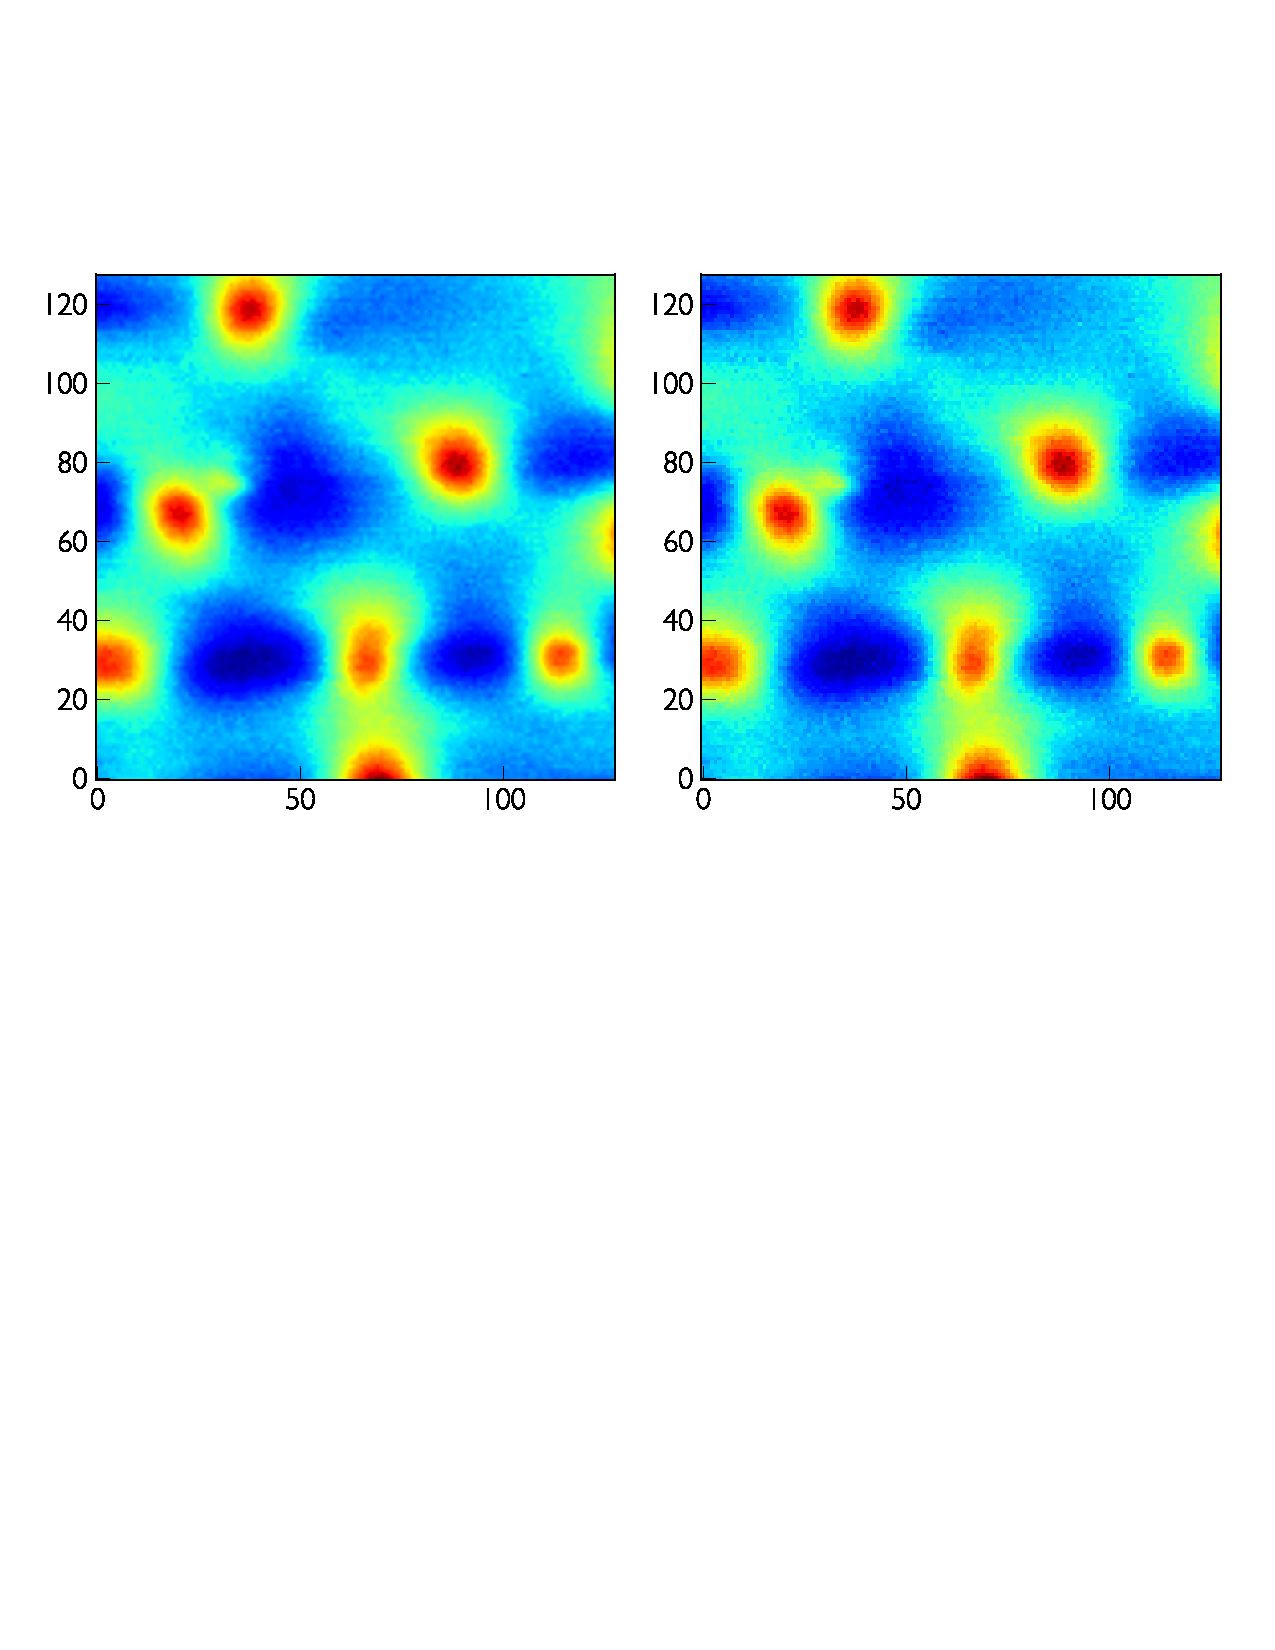
\includegraphics[clip=true,width=\columnwidth]{pixel-compare}
    \caption{Comparison between blurry pixels (dishonest interpolation occurs when the image is processed in Microsoft Powerpoint) vs.\ clean pixels (honest representation is preserved when the image is processed in Python and Adobe Illustrator). MFM images of vortices in NdFeAsO$_{1-x}$F$_x$ \cite{ZhangPRB2015}.}
     \label{fig:pixels}
\end{figure}

\ptitle{Figure file size} Note that faithful representation of images in vector format usually also results in a smaller figures size. This can be important, because the arXiv places an upper bound of 5 MB on each submitted manuscript.

\ptitle{Figure font size} All figure fonts should be at least size \minfont\ in the final publication figure \cite{deBivort}. Note also that san-serif fonts are preferred by most journals (e.g. Arial, Helvetica). To achieve the appropriate font size, please start by measuring the desired final figure size (e.g.\ one or two column width) in the desired journal. Then make a box in Adobe Illustrator (or other program) of exactly the final size, and build your figure within it, using no fonts smaller than size \minfont. Although some journals do prefer that you initially submit your figure at full-page size, you can easily scale up your figure for this purpose. But if you start with a page-size figure and arbitrary font sizes, it becomes harder to later scale it down while maintaining adequate font size.

\vspace{2mm}
\noindent \textbf{Figure checklist:}
\begin{itemize}[label=$\Box$]
\item Use consistent font, at least size \minfont.
\item Label all axes, with units.
\item Each plot should have a legend that describes {\em all} symbols and lines.
\item Each image (or set of same-scale images) should have an accurate length scalebar, with numerical label. (Note that some journals discourage or ``forbid'' superimposing the numerical length on the image. But our goal is clarity: we want the reader to understand the image at a glance, without digging through a lengthy caption to find the necessary number. Journals will generally accept this argument for keeping the number on the image.)
\item Each image (or set of same-palette images) should have a colorbar. The colorbar should be labeled with numerical values and units if possible.
%\item If possible, choose colors that will print well in grayscale. But this is no longer a high priority, since most people read online, or have access to color printers.
\item If using a waterfall plot to display a set of spectra: clearly state the offset of the waterfall plot, or use small horizontal lines to denote the true zero reference for each individual spectrum.
\item The caption should describes all figure sub-parts, in order. Each and every mark on the figure should be described; there should be no mysterious unexplained arrows or other features.
\item If any analysis has been performed (i.e.\ if it's not raw data), then all analysis steps should be clearly divulged, usually in the caption (rather than main text).
\item Clearly explain the origin of all error bars, usually in the caption (rather than main text).
\item For STM images: give setup conditions in the caption ($V_\mathrm{sample}=100$ mV; $R_J=1$ G$\Omega$).
\item For STM spectra: give sample bias modulation in the caption ($V_\mathrm{rms}=2$ mV).
\item For all data: clarify temperature and field conditions in the caption.
\item Appropriately cite all copied figures or data, in the caption of the figure.
\item Use {\tt \textbackslash label\{fig:name\}} within the caption, and use {\tt \textbackslash ref\{fig:name\}} in the paper to refer to it.

\end{itemize}